\section{Convolutional Neural Networks}


\begin{table}[t]
\centering
\begin{tabular}{|l|l|l|l|}
\hline
 & Top-1 & Top-2 & Top-3 \\ \hline
LeNet & 0.20 &  0.40 & 0.60 \\ \hline
GoogleNet &  0.90 & 0.95 & 0.98 \\ \hline
AlexNet &  0.92 & 0.96 & 0.98 \\ \hline
NiN &  0.29 & - & - \\ \hline
\end{tabular}
\caption{The test top-N accuracies of different CNN networks. For LeNet we reported the best accuracy only for comparison purposes due to failing of convergence.}
\label{CNN_test_accuracies}
\end{table}

\begin{table}[t]
\centering
\scriptsize
\begin{tabular}{|l|l|l|l|}
\hline
Layer & Name & Size & Description \\ \hline
0 & INPUT & 227x227x3 & Size 227x227 with 3 channels \\ \hline
1 & CONV1-96 & 55x55x96 & 11x11 filters at stride 4 \\ \hline
2 & MAX POOL & 27x27x96 & 3x3 filters at stride 2 \\ \hline
3 & NORM & 27x27x96 & Normalization \\ \hline
4 & CONV2-256 & 27x27x256 & 5x5 filters at stride 1 \\ \hline
5 & MAX POOL & 13x13x256 & 3x3 filters at stride 2 \\ \hline
6 & NORM & 13x13x256 & Normalization \\ \hline
7 & CONV-384 & 13x13x384 & 384 3x3 filters at stride 1 \\ \hline
8 & CONV-384 & 13x13x384 & 384 3x3 filters at stride 1 \\ \hline
9 & CONV-256 & 13x13x256 & 256 3x3 filters at stride 1 \\ \hline
10 & MAX POOL & 6x6x256 & 3x3 filters at stride 2 \\ \hline
11 & FC6 & 4096 & Fully Connected layer\\ \hline
12 & FC7 & 4096 &  Fully Connected layer \\ \hline
13 & FC8 & \textbf{5} & class numbers \\ \hline
\end{tabular}
\caption{ AlexNet architecture and parameters}
\label{alexnetstructure}
\end{table}

\begin{figure}[t]
\centering
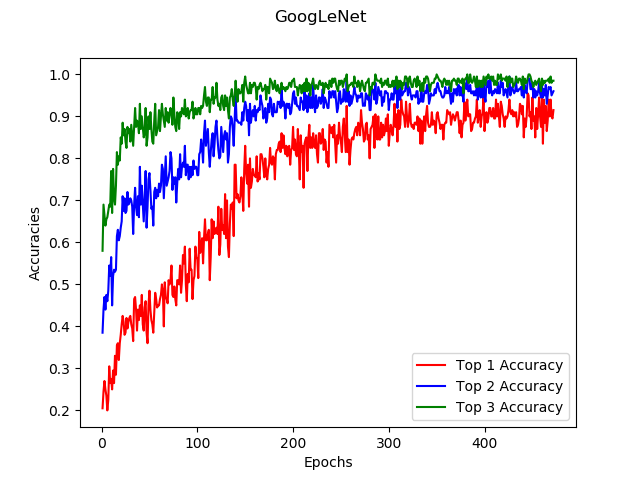
\includegraphics[width=0.4\textwidth]{google_acc.png}
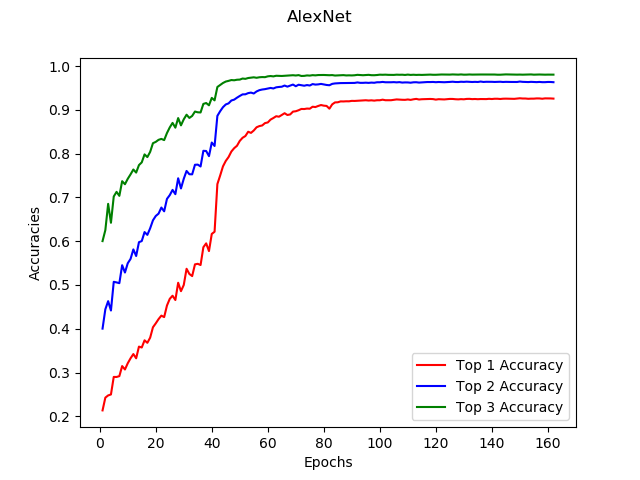
\includegraphics[width=0.4\textwidth]{alex_acc.png}
\caption{Test accuracy vs. epoch numbers for GoogLeNet and AlexNet }
\label{cnn_acc}
\end{figure}

\subsection{Methodology}

We applied different CNN architectures to train 
classifiers from the raw pixels of the images. That is, we transformed  
an image into a 256x256x3 matrix first, where each item in the matrix corresponds 
to a RGB value (without normalization). The classifier took the matrix as input and performed random cropping to fit the input size, 
and further performed predefined data augmentation methods on the matrix. 

We trained four deep models: AlexNet, GoogLeNet, LeNet and Network in Network~(NIN)~
\cite{nin,GoogleNet,LeNet,AlexNet}.
All the parameters were taken from the original papers, except that
we changed the output unit of the networks to 5, corresponding to five classes 
in our case. We showed the structure and parameters we used in AlexNet in \tabref{alexnetstructure}. 
To save space we omitted the parameters of the other models. 

We used Caffe to implement our models. The metrics we considered are training loss 
and test top-N accuracy (N=1,2,3). For top-N accuracy, 
if the target label is in the model's top N predictions with the highest probabilities, 
we consider it as ``correct'', and use the total number of correct classification 
divided by the number of test instances as the top-N accuracy score. 

We fixed the batch size in the training as 200, so it will take 250 iterations to 
complete one epoch. For GoogLeNet, AlexNet and NIN, we set the stepsize to 100,000 (i.e., dropping 
the learning rate every 100\,K iterations) and the momentum to 0.9. The initial 
learning rates are all set to 0.01. We recorded the training loss and test accuracies 
every epoch to examine their trends. 

\begin{figure}[t]
\centering
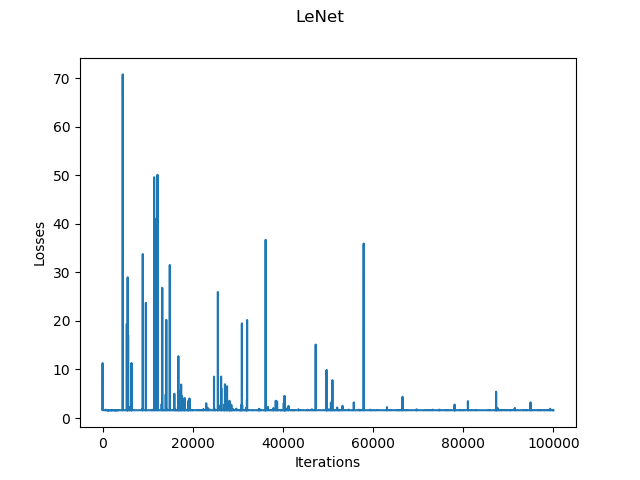
\includegraphics[width=0.4\textwidth]{lenet_loss.png}
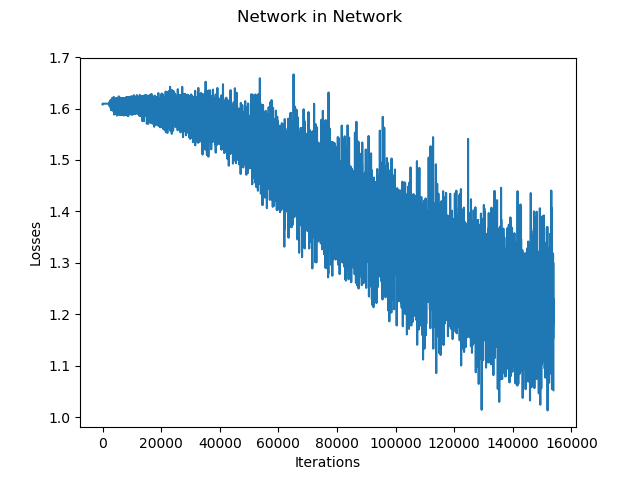
\includegraphics[width=0.4\textwidth]{nin_loss.png}
\caption{Some failures: Loss vs. Iteration for LeNet and Network in Network}
\label{failed_losses}
\end{figure}

\subsection{Evaluation}
A summary of the results can be seen at \tabref{CNN_test_accuracies}. 
On training GoogLeNet and AlexNet, we observe excellent results. For training GoogLeNet, we performed around 120,000 iterations, . We trained AlexNet for 40,000 iterations at a stepsize of 10,000 and the same momentum of 0.9. Compared to the 50-75\% accuracies achieved in the traditional methods, we were able to train our deep NN models of over 90\% accuracy without too much preprocessing (see \figref{cnn_acc}). We note the relative ease with which we could train AlexNet. It took AlexNet only a little more than 20,000 iterations to converge, whereas GoogLeNet required more than 80,000 iterations to achieve similar accuracy (see \figref{cnn_loss}). AlexNet trained faster than an hour using an nVidia GeForce GTX 1080 Titan, whereas GoogNet took us about half a day to fully converge. We count this remarkable behavior toward the simplicity of AlexNet (see \figref{alexnetstructure}), as opposed to the complex inception layout of GoogLeNet (see \figref{googlenet_arch}). 

However, on the other side, we found that CNNs are not a panacea. While testing LeNet and NIN models, we found that both networks fail to converge readily (see \figref{failed_losses}). We did not dig much into why these networks won't work. One possibility for LeNet' failure is that the images are resized to 32x32x3 by the model to cope with its 
input restrictions, therefore many useful information were lost during this processing stage. 
    
\subsection{Discussion}

The simplicity of the machine learning process is obvious when using Deep Convolutional Neural Networks. It allow us to ignore the laborious manual work involved in traditional machine learning methodology such as feature extraction while getting radically better performance. Surprisingly, 
even with relatively small training set (50,000+ images), GoogLeNet and AlexNet can still  
extract high-quality, representative features that can be used to distinguish different classes of images. Our results also show some CNNs might have very good portability and can be even used for domain-specific image~(e.g, medical images) 
classification tasks, as opposed to the suspicions that CNNs are tuned for certain datasets. 



